\sectioncounter{15}
\section{弧度制与任意角的三角函数}

\subsection{知识梳理}
角 (angle) 是由一条射线围绕其端点旋转而成的图形, 旋转开始时的射线为始边, 
旋转中止时的射线为终边, 射线的端点为顶点. 
把角放在平面直角坐标系中, 顶点与原点重合, 始边与 $x$ 轴正半轴重合, 
终边相对 $x$ 轴正半轴逆时针旋转所成的角为正角, 顺时针旋转所成的角为负角, 
角的大小为累计旋转的度数. 由此可知, $x$~轴正半轴表示的角构成集合 
$\{k\cdot360^\circ\mid k\in\mathbb{Z}\}$,  
而第一、三象限角平分线 (直线 $y=x$) 表示的角构成集合
$\{45^\circ+k\cdot180^\circ\mid k\in\mathbb{Z}\}$.

除角度制外, 还可以用弧度制来度量角. 此时将等于半径长的圆弧所对的圆心角大小定义为 $1$~弧度 (radian), 记为 $1\,\mathrm{rad}$,
所以 $360^\circ =2\pi\,\mathrm{rad}$. 由相似性可知, 弧度的大小与所在圆的半径大小无关. 若圆心角 $\alpha$ 所对的弧长为 $l$, 
则其弧度数的绝对值 $|\alpha|=\dfrac{l}{r}$, 其中 $r$ 是圆的半径.
弧度与角度互换公式: 
\[1\,\mathrm{rad}= \Big(\frac{180}{\pi}\Big)^{\circ} \approx 57.3^{\circ}, \quad
    1^{\circ}= \frac{\pi}{180}\,\mathrm{rad}.\]
由弧度的定义可知弧长公式 $l=|\alpha|r$, 而扇形面积公式 (与三角形面积公式类似) 为
\[S= \dfrac{1}{2}lr= \dfrac{1}{2}|\alpha| r^2.\]

如图 \ref{fig-190421-1130} 所示, 设 $\alpha$ 是任意一个角, 顶点为坐标原点, 始边为 $x$ 轴正半轴, 取终边上任意一点 $P(x, y)$ (异于原点), 它到原点的距离 
\[r=|OP|= \sqrt{x^2+ y^2}> 0,\]
那么 
\[\sin\alpha= \frac{y}{r},\quad
    \cos\alpha= \frac{x}{r},\quad 
    \tan\alpha= \frac{y}{x}\ (x\neq 0).\]

\begin{figure}[hb]
    \centering\small
    \begin{tikzpicture}[scale=1.1]
        \draw[-{Stealth[scale=0.8]}] (-1.2,0) -- (1.4,0) node[below] {$x$};
        \draw[-{Stealth[scale=0.8]}] (0,-1.2) -- (0,1.3) node[left] {$y$};
        \draw (0,0) circle (1) node[anchor=45] {$O$} coordinate (O);

        \def\myangle{40};
        \pgfmathparse{tan(\myangle)};
        \coordinate (B) at (\myangle:1.6);
        \draw[fill=black] (1,0) circle (0.6pt) coordinate (A)
        +(0.1,0) node[below] {$A$};
        \draw[fill=black] (1,\pgfmathresult) coordinate (T) circle (0.6pt) 
        node[above] {$T$} ;
        \draw[fill=black] (\myangle:1) circle (0.6pt) coordinate (P)
        +(0,0.06) node[above] {$P$};
        \draw[fill=black] ($(O)!(P)!(A)$) coordinate (M) circle (0.6pt) 
        node[below] {$M$};
        \draw (O)--(B) (M)--(P) (A)--(T);      
    \end{tikzpicture}
    \caption{}\label{fig-190421-1130}
\end{figure}

三角函数值只与角的大小有关, 而与终边上点~$P$ 的位置无关. 由定义容易判断各象限内的角的三角函数值的正负号. 若点~$P$ 恰在单位圆 (圆心为原点且半径为 $1$) 上, 取点~$A(1,0)$, 并作 $PM\perp OA$ 于点 $M$, 作 $TA\perp OA$ 并交射线~$OP$ 于点~$T$, 则此时 $r=1$, 且
\[\sin\alpha= y,\quad
    \cos\alpha= x,\quad 
    \tan\alpha= \frac{AT}{OA}= AT\ (x\neq 0).\]
对 $\angle{POA}$ 来说, $MP$ 为正弦线, $OM$ 为余弦线, $AT$ 为正切线, 
且各线段均为有向线段 (与向量类似). 

常用的特殊角的三角函数值, 参考图~\ref{fig-190421-1140}. 由此可以写出其他特殊角 ($120^\circ$, $135^\circ$, $150^\circ$ 等) 的各三角函数值. 写三角函数值时, 通常省略弧度单位, 如
\[\begin{gathered}
    \sin30^\circ= \sin\frac{\pi}6= \frac12,\\
    \cos135^\circ= \cos\frac{3\pi}4= -\frac{\sqrt2}2.
\end{gathered}\] 

\begin{figure}[hb]
    \centering\small
    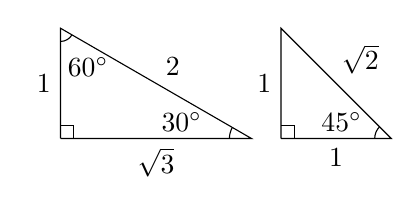
\begin{tikzpicture}[scale=1.4]
        \pgfmathparse{sqrt(3)};
        \draw (0,0) coordinate (A)-- node[below] {$\sqrt3$} 
        (1.732,0) coordinate (B)-- node[anchor=225] {$2$}
        (0,1) coordinate (C)--node[left] {$1$} (0,0);
        \draw (A)++(0,0.12)--++(0.12,0)--++(0,-0.12);
        \draw (C)+(0,-0.12) arc (270:330:0.12);
        \draw (B)+(-0.2,0) arc (180:150:0.2);
        \draw (A)+(0.25,0.65) node {$60^\circ$} +(1.1,0.15) node {$30^\circ$};
        \draw (2,0) coordinate (D)-- node[below] {$1$} 
        +(1,0) coordinate (E)-- node[anchor=225] {$\sqrt2$}
        +(0,1) coordinate (F)--node[left] {$1$} (D);
        \draw (D)++(0,0.12)--++(0.12,0)--++(0,-0.12);
        \draw (E)+(-0.15,0) arc (180:135:0.15);
        \draw (D)+(0.55,0.15) node {$45^\circ$};
    \end{tikzpicture}
    \caption{}\label{fig-190421-1140}
\end{figure}

\lianxi
\begin{exercise}
    判断 $\sin6$ 的正负号.
\end{exercise}
\beginsolution
    题中的 $6$ 表示 $6\,\mathrm{rad}$.
    \mymarginpar{同理可知,
    \[\sin 1>0,\ \cos 2<0,\ \tan 3<0.\]}
    因为
    \[\begin{gathered}
        270^\circ= \frac{3\pi}2\,\mathrm{rad}
            \approx 4.71\,\mathrm{rad},\\
        360^\circ= 2\pi\,\mathrm{rad}
            \approx 6.28\,\mathrm{rad},\\
    \end{gathered}\]
    所以 $6\,\mathrm{rad}$ 为第四象限角. 由正弦线知, $\sin 6<0$.
\endsolution

\begin{exercise}
    求终边落在直线 $y=-x$ 上的角 $\alpha$ 的集合.
\end{exercise}
\beginsolution
    因为直线 $y=-x$ 为第二、四象限的角平分线, 
    \mymarginpar{类似的还有 ($k\in\mathbb{Z}$), \\
    \[\begin{gathered}
        y=\sqrt3x\Leftrightarrow \alpha=\frac\pi3+k\pi,\\
        y=-\sqrt3x\Leftrightarrow \alpha=\frac{2\pi}3+k\pi,\\
        y=\frac{\sqrt3}3 x\Leftrightarrow 
            \alpha=\frac\pi6+k\pi.
    \end{gathered}\]}
    所以所求集合为
    \[\begin{aligned}
        &\{\alpha\mid \alpha= 135^\circ+ k\cdot 180^\circ,\ k\in\mathbb{Z}\}\\
        ={}& \biggl\{\alpha\Bigm| \alpha= \frac{3\pi}{4}+ k\pi,\ k\in\mathbb{Z}\biggr\}.
    \end{aligned}\]
    以上两种写法均可, 后一种写法略微简洁一些.
\endsolution

\begin{exercise}
    已知某扇形的半径为 $10$, 面积为 $\dfrac{50\pi}3$, 求该扇形的圆心角大小.
\end{exercise}
\beginsolution
    设该扇形半径为 $r$, 圆心角为 $\alpha$, 面积为 $S$, 则 $r=10$. 利用由弧度制表示的扇形面积公式, 
    \[S= \frac12\alpha r^2= \dfrac{50\pi}3,\quad
        \text{解得}\quad
        \alpha= \frac\pi3.\]
\endsolution

\begin{exercise}
    已知角 $\alpha$ 的终边经过点 $P(x,-12)$,  且 $\cos\alpha= -\dfrac5{13}$, 求 $x$ 的值.
\end{exercise}

\beginsolution
    由余弦函数的定义, 
    \mymarginpar{根式方程必须验根, 因为利用平方去掉根号时, 可能产生增根.}
    \[\cos\alpha= \frac{x}{\sqrt{x^2+(-12)^2}}= -\dfrac5{13},\]
    解得 $x=\pm5$. 检验可知, $x=-5$.
\endsolution

\subsection{要点导学\quad 各个击破}
\subsubsection{象限角的表示}

\begin{example}
    已知 $\alpha= 30^\circ$, $\beta= 60^\circ$, $\gamma= 300^\circ$. 如图 \ref{fig-190421-1430} 所示, 在坐标系中表示时, $\alpha$, $\beta$, $\gamma$ 的终边分别是 $OA$, $OB$, $OC$.
  
    (1) 分别写出两图中阴影部分(含边界)的所有角的集合;
  
    (2) 写出右图中阴影部分在 $[0^\circ,360^\circ]$ 上的所有角的集合.
    \begin{figure}[h]
    \small
    \centering
    \begin{tikzpicture}
    \draw[-{Stealth[scale=0.8]}] (-1.3,0) -- (1.5,0) node[below] {$x$};
    \draw[-{Stealth[scale=0.8]}] (0,-1.3) -- (0,1.5) node[left] {$y$};
    \draw (0,0) node[anchor=135] {$O$} coordinate (O);
    \draw (30:1.2)  coordinate (A) node[right] {$A$};
    \draw (210:1.2)  coordinate (A');
    \draw (60:1.2)  coordinate (B) node[above] {$B$};
    \draw (240:1.2) coordinate (B');
    \draw[line width=0.6pt] (A)--(A') (B)--(B');
    \draw[fill=black!30,line width=0pt] (A)--(O)--(B)--cycle;
    \draw[fill=black!30,line width=0pt] (A')--(O)--(B')--cycle;
    \end{tikzpicture}\hskip 1cm
    \begin{tikzpicture}
    \draw[-{Stealth[scale=0.8]}] (0,-1.3) -- (0,1.5) node[left] {$y$};
    \draw (0,0) node[anchor=45] {$O$} coordinate (O);
    \draw (30:1.2)  coordinate (A) node[right] {$A$};
    \draw (300:1.2)  coordinate (C) node[right] {$C$};
    \draw[line width=0.6pt] (A)--(O)--(C);
    \draw[fill=black!30,line width=0pt] (A)--(O)--(C)--cycle;
    \draw[-{Stealth[scale=0.8]}] (-0.5,0) -- (1.5,0) node[below] {$x$};
    \end{tikzpicture}
    \caption{}\label{fig-190421-1430}
    \end{figure}
\end{example}
\beginsolution
    (1) 写角的集合时, 应简洁且各段连续, 并注意周期性. 前者为
    \[\{\theta\mid 30^\circ+k\cdot 180^\circ\leqslant \theta
        \leqslant 60^\circ+k\cdot 180^\circ,\ 
        k\in\mathbb{Z}\},\]
    后者为
    \[\{\theta\mid -60^\circ+k\cdot 360^\circ\leqslant \theta
        \leqslant 30^\circ+k\cdot 360^\circ,\ 
        k\in\mathbb{Z}\},\]
    
    (2) $[0^\circ,30^\circ]\cup [300^\circ,360^\circ]$.
\endsolution

\lianxi
\begin{exercise}
    终边落在坐标轴上的角的集合如何表示\,?
\end{exercise}
\beginsolution
    $\biggl\{\alpha\Bigm| \alpha= \dfrac{k\pi}2,\ k\in\mathbb{Z}\biggr\}$.
\endsolution

\begin{exercise}
    若角 $\beta$ 的终边与 $\alpha= \dfrac{\pi}6$ 的终边关于直线 $y=x$ 对称, 求角 $\beta$ 的集合.
\end{exercise}
\beginsolution
    由草图知, 可先设 $\beta$ 为锐角, 即 $\beta\in\biggl[0,\dfrac\pi2\biggr]$. 因为直线 $y=x$ 为第一、三象限的角平分线, 所以
    \[\frac{\alpha+ \beta}2= \frac{\pi}4,\quad
        \text{解得}\quad \beta= \frac\pi3.\]
    再考虑一般情形可知, 所求的集合为
    \[\biggl\{\beta\Bigm| \beta= \dfrac{\pi}3+ 2k\pi,\ 
        k\in\mathbb{Z}\biggr\}.\]
\endsolution

\subsubsection{任意角的三角函数}
\begin{example}
    已知角 $\alpha$ 的终边经过点 $P(-\sqrt3,y)$ ($y\neq0$), 且 $\sin\alpha =\dfrac{\sqrt2}4 y$, 求 $\cos \alpha$ 和 $\tan\alpha$ 的值.
\end{example}
\beginsolution
    由正弦函数的定义,
    \[\sin\alpha= \frac{y}{\sqrt{(-\sqrt3)^2+ y^2}}
        = \dfrac{\sqrt2}4 y,\]
    解得 $y= \pm\sqrt5$, 且均合题意. 当 $y=\sqrt5$ 时,
    \[\begin{gathered}
        \cos\alpha= \frac{-\sqrt3}{\sqrt8}
            = -\frac{\sqrt6}{4},\\
        \tan\alpha= \frac{\sqrt5}{-\sqrt3}
            = -\frac{\sqrt{15}}{3}.
    \end{gathered}\]
    同理可知, 当 $y= -\sqrt5$ 时, $\cos\alpha= -\frac{\sqrt6}{4}$, $\tan\alpha= \frac{\sqrt{15}}{3}$.
\endsolution

\lianxi
\begin{exercise}[s]
    已知角 $\alpha$ 的终边过点 $P(-4a,3a)$ ($a\neq0$), 求 $2\sin\alpha +\cos\alpha$ 的值.
\end{exercise}
\beginsolution
    点 $P$ 到原点 $O$ 的距离
    \[|OP|= \sqrt{(-4a)^2+ (3a)^2}= 5|a|.\]

    (1) 若 $a>0$, 则 $|OP|= 5a$, 
    \[\sin\alpha= \frac{3a}{|OP|}= \frac35,\quad
        \cos\alpha= \frac{-4a}{|OP|}= -\frac45,\]
    所以 
    \[2\sin\alpha +\cos\alpha
        = 2\cdot \frac35+ \biggl(-\frac45\biggr)
        = \frac25.\]

    (2) 若 $a>0$, 则 $|OP|= 5a$, 同理可得
    \[2\sin\alpha +\cos\alpha= -\frac25.\]
\endsolution

\subsubsection{扇形的基本运算}
\begin{example}
    若扇形圆心角为 $120^\circ$, 半径为 6\,cm, 求该扇形的弧长及所含弓形的面积.
\end{example}
\beginsolution
    此题利用弧度制时计算量会小一些. 设该扇形的半径为 $r$, 弧长为 $l$. 因为 $120^\circ= \dfrac{2\pi}{3}\,\mathrm{rad}$, 所以
    \[l= \alpha r= \dfrac{2\pi}{3}\cdot 6= 4\pi\,(\mathrm{cm}).\]
    画图可知, 弓形的面积等于扇形的面积减去三角形的面积, 
    \mymarginpar{此处用了三角形面积定理, 也可以直接用三角形面积公式 (底乘高的一半).}
    故
    \[\begin{aligned}
        S_{\text{弓形}}
        &= S_{\text{扇形}}- S_{\text{三角形}}
            = \frac12\alpha r^2- \frac12\sin\alpha r^2\\
        &= \frac12\biggl(\frac{2\pi}{3}- \sin\frac{2\pi}{3}\biggr)\cdot 6^2
            = 3(4\pi- 3\sqrt3)\,(\mathrm{cm}^2).
    \end{aligned}\]
\endsolution

\lianxi
\begin{exercise}[s]
    若扇形的周长为 $20$, 求此扇形的面积最大值.
\end{exercise}
\beginsolution
    设此扇形半径为 $r$, 弧长为 $l$, 面积为 $S$, 则 $2r+l=20$, 且
    \[S= \frac12lr= \frac12(20-2r)\cdot r
        = (10-r)r.\]
    当 $r=5$ 时, $S=25$ 最大. 
    \mymarginpar{扇形的圆心角 $\alpha\in(0,2\pi)$.}
    此时 $l=10$, 圆心角大小为 $\dfrac{l}r= 2\,\mathrm{rad}$, 符合题意.
\endsolution

\subsubsection{课堂评价}
\begin{exercise}
    下列命题中正确的是\,? (填序号)
  
    (1) 终边相同的角一定相等;
  
    (2) 锐角都是第一象限的角;
  
    (3) 角 $\alpha$ 与角 $2\alpha$ 的终边一定不相同;
  
    (4) 第二象限的角一定大于第一象限的角.
\end{exercise}
\beginsolution
    (1) 不正确, 可能大小相差 $2k\pi$, $k\in\mathbb{Z}$.

    (2) 由定义知, 正确.

    (3) 不正确. 当 $\alpha=2k\pi$, $k\in\mathbb{Z}$ 时, $\alpha=4k\pi$, 终边均为 $x$ 轴正半轴.

    (4) 不正确. 取第二象限的角 $120^\circ$, 第一象限的角 $30^\circ+360^\circ= 390^\circ$, 可知结论不成立.
\endsolution

\begin{exercise}
    若 $120^\circ$ 的角的终边上有一点 $(-4,a)$, 求 $a$ 的值.
\end{exercise}
\beginsolution
    由 $\tan120^\circ= \dfrac{a}{-4}= -\sqrt3$ 解得 $a=4\sqrt3$.
\endsolution

\begin{exercise}
    已知 $\alpha$ 的终边在直线 $y=2x$ 上, 求 
    $\dfrac{\sin\alpha+ \cos\alpha}{\sin\alpha-\cos\alpha} +\tan\alpha$ 的值.
\end{exercise}
\beginsolution
    直接利用 $\tan\alpha$ 的值.
    \mymarginpar{也可以分别考虑 $\alpha$ 在第一、三象限的情况, 并计算对应的 $\sin\alpha$, $\cos\alpha$ 和 $\tan\alpha$.}
    因为 $\tan\alpha= \dfrac{y}{x}= 2$, 而
    \[\begin{aligned}
        \frac{\sin\alpha+ \cos\alpha}{\sin\alpha-\cos\alpha}
        &= \frac{\dfrac{\sin\alpha}{\cos\alpha}+ 1}{\dfrac{\sin\alpha}{\cos\alpha}- 1}
        = \frac{\tan\alpha+ 1}{\tan\alpha- 1}\\
        &= \frac{2+1}{2-1}= 3,
    \end{aligned}\]
    所以所求式子的值为 $3+2=5$. 
\endsolution

\begin{exercise}
    若扇形的周长是 $6\,\mathrm{cm}$, 面积是 $2\,\text{cm}^2$, 求该扇形圆心角的大小.
\end{exercise}
\beginsolution
    设该扇形的半径为 $r$, 弧长为 $l$, 则
    \[\left\{\!\!\begin{array}{l}
        2r+l= 6,\\
        \dfrac12rl= 2,
    \end{array}\right.\ \text{解得}\ 
    \left\{\!\!\begin{array}{l}
        r=2,\\
        l=2,
    \end{array}\right.\text{或}\ 
    \left\{\!\!\begin{array}{l}
        r=1,\\
        l=4,
    \end{array}\right.\]
    所以圆心角大小为 $\dfrac{l}r= 1\,\mathrm{rad}$ 或 $4\,\mathrm{rad}$.
\endsolution

\subsection{课后练习}

\begin{exercise}
    用 $\alpha$ 表示与其终边关于 $x$ 轴对称的角的集合.
\end{exercise}
\beginsolution
    $\{\beta\mid \beta= -\alpha+ 2k\pi,\ k\in\mathbb{Z}\}$.
\endsolution

\begin{exercise}
    已知角 $\alpha$ 的终边上有一点 $P(12a,5a)$, 其中 $a<0$, 
    求 $\sin\alpha$ 的值.
\end{exercise}
\beginsolution
    因为 $a<0$, 所以
    \[\begin{gathered}
        |OP|= \sqrt{(12a)^2+ (5a)^2}= 13|a|= -13a,\\
        \sin\alpha= \frac{5a}{|OP|}= \frac{5a}{-13a}
            = -\frac{5}{13}.
    \end{gathered}\]
\endsolution

\begin{exercise}
    若角 $\theta$ 终边上一点 $P(x,3)$ ($x\neq 0$), 
    且 $\cos\theta = \dfrac{\sqrt{10}}{10} x$, 求 $\sin\theta$ 的值.
\end{exercise}
\beginsolution
    由 $\cos\theta= \dfrac{x}{\sqrt{x^2+3^2}}= \dfrac{\sqrt{10}}{10} x$ 解得 $x=\pm1$, 均合题意. 所以, 当 $x=1$ 时,
    \[\sin\theta= \dfrac{3}{\sqrt{10}}= \frac{3\sqrt{10}}{10};\]
    当 $x=-1$ 时, $\sin\theta= -\frac{3\sqrt{10}}{10}$.
\endsolution

\begin{exercise}
    若扇形的周长是 $8\,\mathrm{cm}$, 面积为 $4\,\text{cm}^2$, 
    求该扇形圆心角的大小.
\end{exercise}
\beginsolution
    设该扇形的半径为 $r$, 弧长为 $l$, 则
    \[\left\{\!\!\begin{array}{l}
        2r+l= 8,\\
        \dfrac12rl= 4,
    \end{array}\right.\ \text{解得}\ 
    \left\{\!\!\begin{array}{l}
        r=2,\\
        l=4,
    \end{array}\right.\]
    所以圆心角大小为 $\dfrac{l}r= 2\,\mathrm{rad}$.
\endsolution

\begin{exercise}
    设集合 $M=\biggl\{x\Bigm| x=\sin\dfrac{n\pi}3,\ n\in\mathbb{Z}\Big\}$, 求满足条件 $P\cup\biggl\{\dfrac{\sqrt3}2, -\dfrac{\sqrt3}2\biggr\}=M$ 的集合 $P$ 的个数.
\end{exercise}
\beginsolution
    由正弦线知, 
    \mymarginpar{一般地, 若集合
    \[\begin{aligned}
        M&=\{a_1,a_2,\cdots,a_n\},\\
         &=P\cup\{a_1,a_2,\cdots,a_m\}
    \end{aligned}\]
    且 $m<n$, 则满足条件的 $P$ 的个数为 $2^{n-m}$.}
    $M=\biggl\{0,\dfrac{\sqrt3}2,-\dfrac{\sqrt3}2\biggr\}$, 所以集合 $P$ 中必含元素 $0$, 而 $\dfrac{\sqrt3}2$, $-\dfrac{\sqrt3}2$ 为其可选元素, 共 $2^2=4$ 种可能.

    \varexercise 若题中 $M=\biggl\{x\Bigm| x=\sin\dfrac{n\pi}6,\ n\in\mathbb{Z}\Big\}$, 则答案不变.

    \varexercise 若题中 $M=\biggl\{x\Bigm| x=\sin\dfrac{n\pi}6,\ n\in\mathbb{Z}\Big\}$, $P\cup\biggl\{0, \dfrac{\sqrt3}2, -\dfrac{\sqrt3}2\biggr\}=M$, 则答案改为 $2^n$ (为什么?).
\endsolution

\begin{exercise}
    圆心角为 $60^\circ$ 的扇形, 它的弧长为 $2\pi$, 求其内切圆的半径.
\end{exercise}
\beginsolution
    如图 \ref{fig:2021-0214-0900} 所示, 在扇形 $AOB$ 中,
    \mymarginpar{\begin{center}
        \includegraphics[align=u,scale=1.4]{2021-0214-0900-crop}
        \figcaption{}\label{fig:2021-0214-0900}
    \end{center}}
    $\angle AOB= 60^\circ= \dfrac{\pi}3$, 弧 $AB$ 的长 $l=2\pi$. 设 $OA=R$, 则
    \[R=\frac{l}{\angle AOB}= \frac{2\pi}{\pi/3}= 6.\]
    圆 $M$ 与扇形 $AOB$ 相切于点 $N$, $P$, $Q$. 连接 $ON$, 由对称性知, $ON$ 必过点 $M$, 且 $\angle BON= \dfrac12\angle BOA= 30^\circ$. 再连接 $MP$ 并设 $MP=r$, 则 $MP\perp OB$,
    \[MN=r,\quad OM= 2MP= 2r,\]
    所以
    \[ON= OM+MN= 3r.\]
    由 $ON= R= 6$ 知 $r=2$, 此即所求内切圆半径.

    \varexercise 若圆心角改为 $90^\circ$, 则 $OM=\sqrt2 r$,
    \[ON= OM+MN= (\sqrt2+1)r= R,\]
    解得 $r= (\sqrt2-1)R$.

    \varexercise 更一般地, 若圆心角改为 $2\alpha$, 则考虑 $\mathrm{Rt}\triangle OMP$ 知, $\dfrac{OP}{OM}= \sin\alpha$, 故有
    \[R=\biggl(1+\dfrac1{\sin\alpha}\biggr)r.\]
\endsolution

\begin{exercise}
    (1) 已知角 $\alpha$ 的终边上一点 $P(4t,-3t)$ ($t\neq0$),
    求 $2\sin\alpha +\cos\alpha$ 的值;
  
    (2) 已知角 $\beta$ 的终边在直线 $y=\sqrt3x$ 上, 求 $\sin\beta$ 的值.
\end{exercise}
\beginsolution
    (1) 因为 $|OP|=\sqrt{(4t)^2+(-3t)^2}= 5|t|$, 所以当 $t>0$ 时, $|OP|= 5t$,
    \[\sin\alpha= \frac{-3t}{|OP|}= -\frac35,\quad
        \cos\alpha= \frac{4t}{|OP|}= \frac45,\]
    此时
    \[2\sin\alpha +\cos\alpha
        = 2\biggl(-\frac35\biggr)+ \frac45
        = -\frac25.\]
    同理可知, 当 $t>0$ 时, $2\sin\alpha +\cos\alpha= \frac25$.

    (2) 在 $\beta$ 的终边上任取一点 $Q(x,\sqrt3x)$ ($x\neq0$), 则
    \[|OP|=\sqrt{x^2+(\sqrt3x)^2}= 2|x|.\]
    若 $\beta$ 在第一象限, 则 $x>0$, $|OP|= 2x$,
    \[\sin\beta= \frac{\sqrt3x}{|OP|}
        = \frac{\sqrt3x}{2x}= \frac{\sqrt{3}}2.\]
    同理可知, 若 $\beta$ 在第三象限, 则 $\sin\beta=-\frac{\sqrt{3}}2$.
\endsolution